\chapter{Mechanizmy bezpieczeństwa aplikacji internetowych opartych na języku JavaScript}

\section{Wprowadzenie}
W poniższym rozdziale przedstawiono najważniejsze mechanizmy bezpieczeństwa wykorzystywane w aplikacjach internetowych opartych na języku \textit{JavaScript}. Działanie mechanizmów poparto przykładami pochodzącymi z aplikacji internetowej napisanej w ramach pracy magisterskiej. 

\subsection{Komunikacja klient-serwer przy użyciu protokołu HTTPS}
Protokół HTTPS (\textit{Hypertext Transfer Protocol Secure}) jest szyfrowaną wersją protokołu HTTP (\textit{Hypertext Transfer Protocol}). Komunikacja nie jest oparta bezpośrednio na modelu klient-serwer, tylko na zasadzie szyfrowanego protokołu SSL (\textit{Secure Socket Layer}). Dzięki takiemu rozwiązaniu nie ma możliwości przejęcia czy też naruszenia integralności danych przesyłanych w trakcie transmisji. SSL wykorzystuje tzw. certyfikaty mające na celu poświadczenie wiarygodności domeny, bądź domeny oraz jej właściciela. Dzięki temu użytkownik, który korzysta ze strony WWW ma pewność, że przesyłane informacje nie zostaną przechwycone i nie trafią w nieporządane ręce. W momencie nawiązywania połączenia przez przeglądarkę internetową zabezpieczoną protokołem SSL następuje ustalenie odpowiednich algorytmów oraz kluczy szyfrujących, stosowanych następnie do wymiany danych między przeglądarką a serwerem WWW. Wykorzystywana jest tutaj kryptografia asymetryczna o ustalonej długości klucza.

Inicjalizacja serwera w aplikacji rozpoczyna się od wygenerowania klucza i certyfikatu SSL. Można to wykonać za pomocą następującej komendy:

\begin{verbatim}
openssl req -newkey rsa:2048 -new -nodes -keyout key.pem -out cert.pem
\end{verbatim}

Taka komenda generuje nowy certyfikat oraz klucz prywatny RSA (o rozmiarze podanym w bitach) i zapisuje je do plików \textit{key.pem} oraz \textit{cert.pem}. W tym przypadku jest to 2048 bitowy klucz. Zawartość tych plików zostanie przekazana jako parametr metody \texttt{createServer([options], [requestListener])} pakietu NPM o nazwie \textit{https} służącej do zainicjalizowania serwera nasłuchującego na wybranym porcie. Powodem wybrania 2048 bitowego klucza był fakt, iż niektóre urządzenia nie większych wartości bitowych. Ponadto, wykorzystanie tych kluczy podczas szyfrowania i uwierzytelniania pozwala na znacznie mniejsze zużycie procesora.

\newpage
Zawartość wygenerowanych plików przedstawiono na rysunku \ref{Rys:keyandpem}.

\begin{figure}[h]
	\centering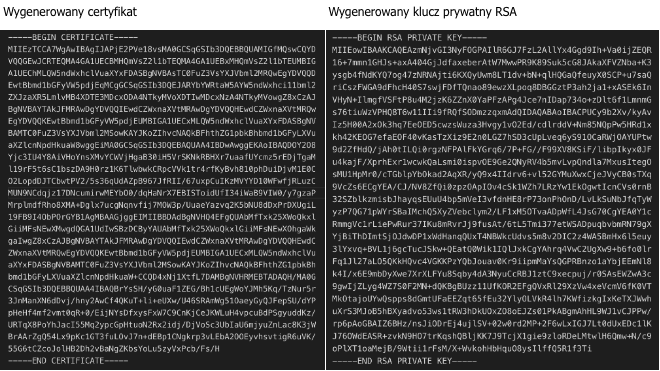
\includegraphics[scale=0.6]{images/security/key_and_certificate.png}
	\caption{Zdjęcie przedstawiające wygenerowany za pomocą komendy \textit{openssl -newkey} certyfikat SSL oraz klucz prywatny RSA.}
	\label{Rys:keyandpem}
\end{figure}

Na rysunku poniżej przedstawiono ogólny schemat działania protokołu HTTPS z wykorzystaniem protokołu SSL podczas wymiany zaszyfrowanych danych między klientem a serwerem:

\begin{figure}[h]
	\centering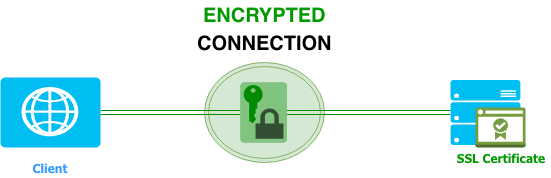
\includegraphics[scale=0.6]{images/security/how-https-works.png}
	\caption{Schemat działania protokołu HTTPS wykorzystującego protokół SSL w trakcie wymiany zaszyfrowanych danych między klientem a serwerem}
	\label{Rys:keyandpem}
\end{figure}

\subsection{Zasady tworzenia haseł użytkowników}
Hasła są obecnie jedną z najpopularniejszych technik uwierzytelniania w Internecie. Jest to metoda bardzo bezpieczna pod warunkiem spełnienia określonych kryteriów. Hasło użytkownika powinno charakteryzować się tym iż nie jest ono ciągiem składającym się z mniej niż dziesięciu znaków. Dzięki takiemu rozwiązaniu liczba możliwych kombinacji (na przykład przy ataku słownikowym) diametralnie wzrasta. Kolejną kwestią jest wykorzystywanie przez użytkowników różnych typów znaków alfanumerycznych - dużych i małych liter, znaków specjalnych oraz cyfr. Znacznie podnosi to poziom skomplikowania zabezpieczenia. 

Twórcy aplikacji internetowych mają dostęp do szeregu bibliotek i pakietów umożliwiających definiowanie reguł tworzenia bezpiecznych haseł użytkowników. W projekcie wykorzystano pakiet NPM o nazwie \textit{password-validator}. Pozwala on na proste definiowanie zasad kreowania haseł i dostarcza mechanizmy weryfikacji czy powyższe zasady zostały spełnione. 

W przykładowym projekcie posłużono się następującymi definicjami reguł:

\begin{verbatim}
schema
.is().min(10)                                   // Minimum length 10
.has().uppercase()                              // Must have uppercase letters
.has().lowercase()                              // Must have lowercase letters
.has().digits()                                 // Must have digits
.has().not().spaces()                           // Should not have spaces
.is().not().oneOf(['Passw0rd', 'Password123', '123456', '123456789', 'qwerty']); 
// Blacklist these values
\end{verbatim}
 
Jak widać, istnieje również możliwość zdefiniowania tzw. \textit{blacklisty} zawierającej najczęściej używane hasła, będące łatwym elementem do wykorzystania podczas na przykład ataku słownikowego. Do walidacji poprawności przesyłanych przez użytkownika haseł wykorzystano metodę oferowaną przez pakiet \textit{password-validator}:

\begin{verbatim}
schema.validate(password, options?)
\end{verbatim}

W przypadku wpisania przez użytkownika hasła nie spełniającego wymagań zdeklarowanych w poniższym schemacie następuje walidacja formularza rejestracji i powiadomienie użytkownika jakie błędy popełnił:

\begin{figure}[h]
	\centering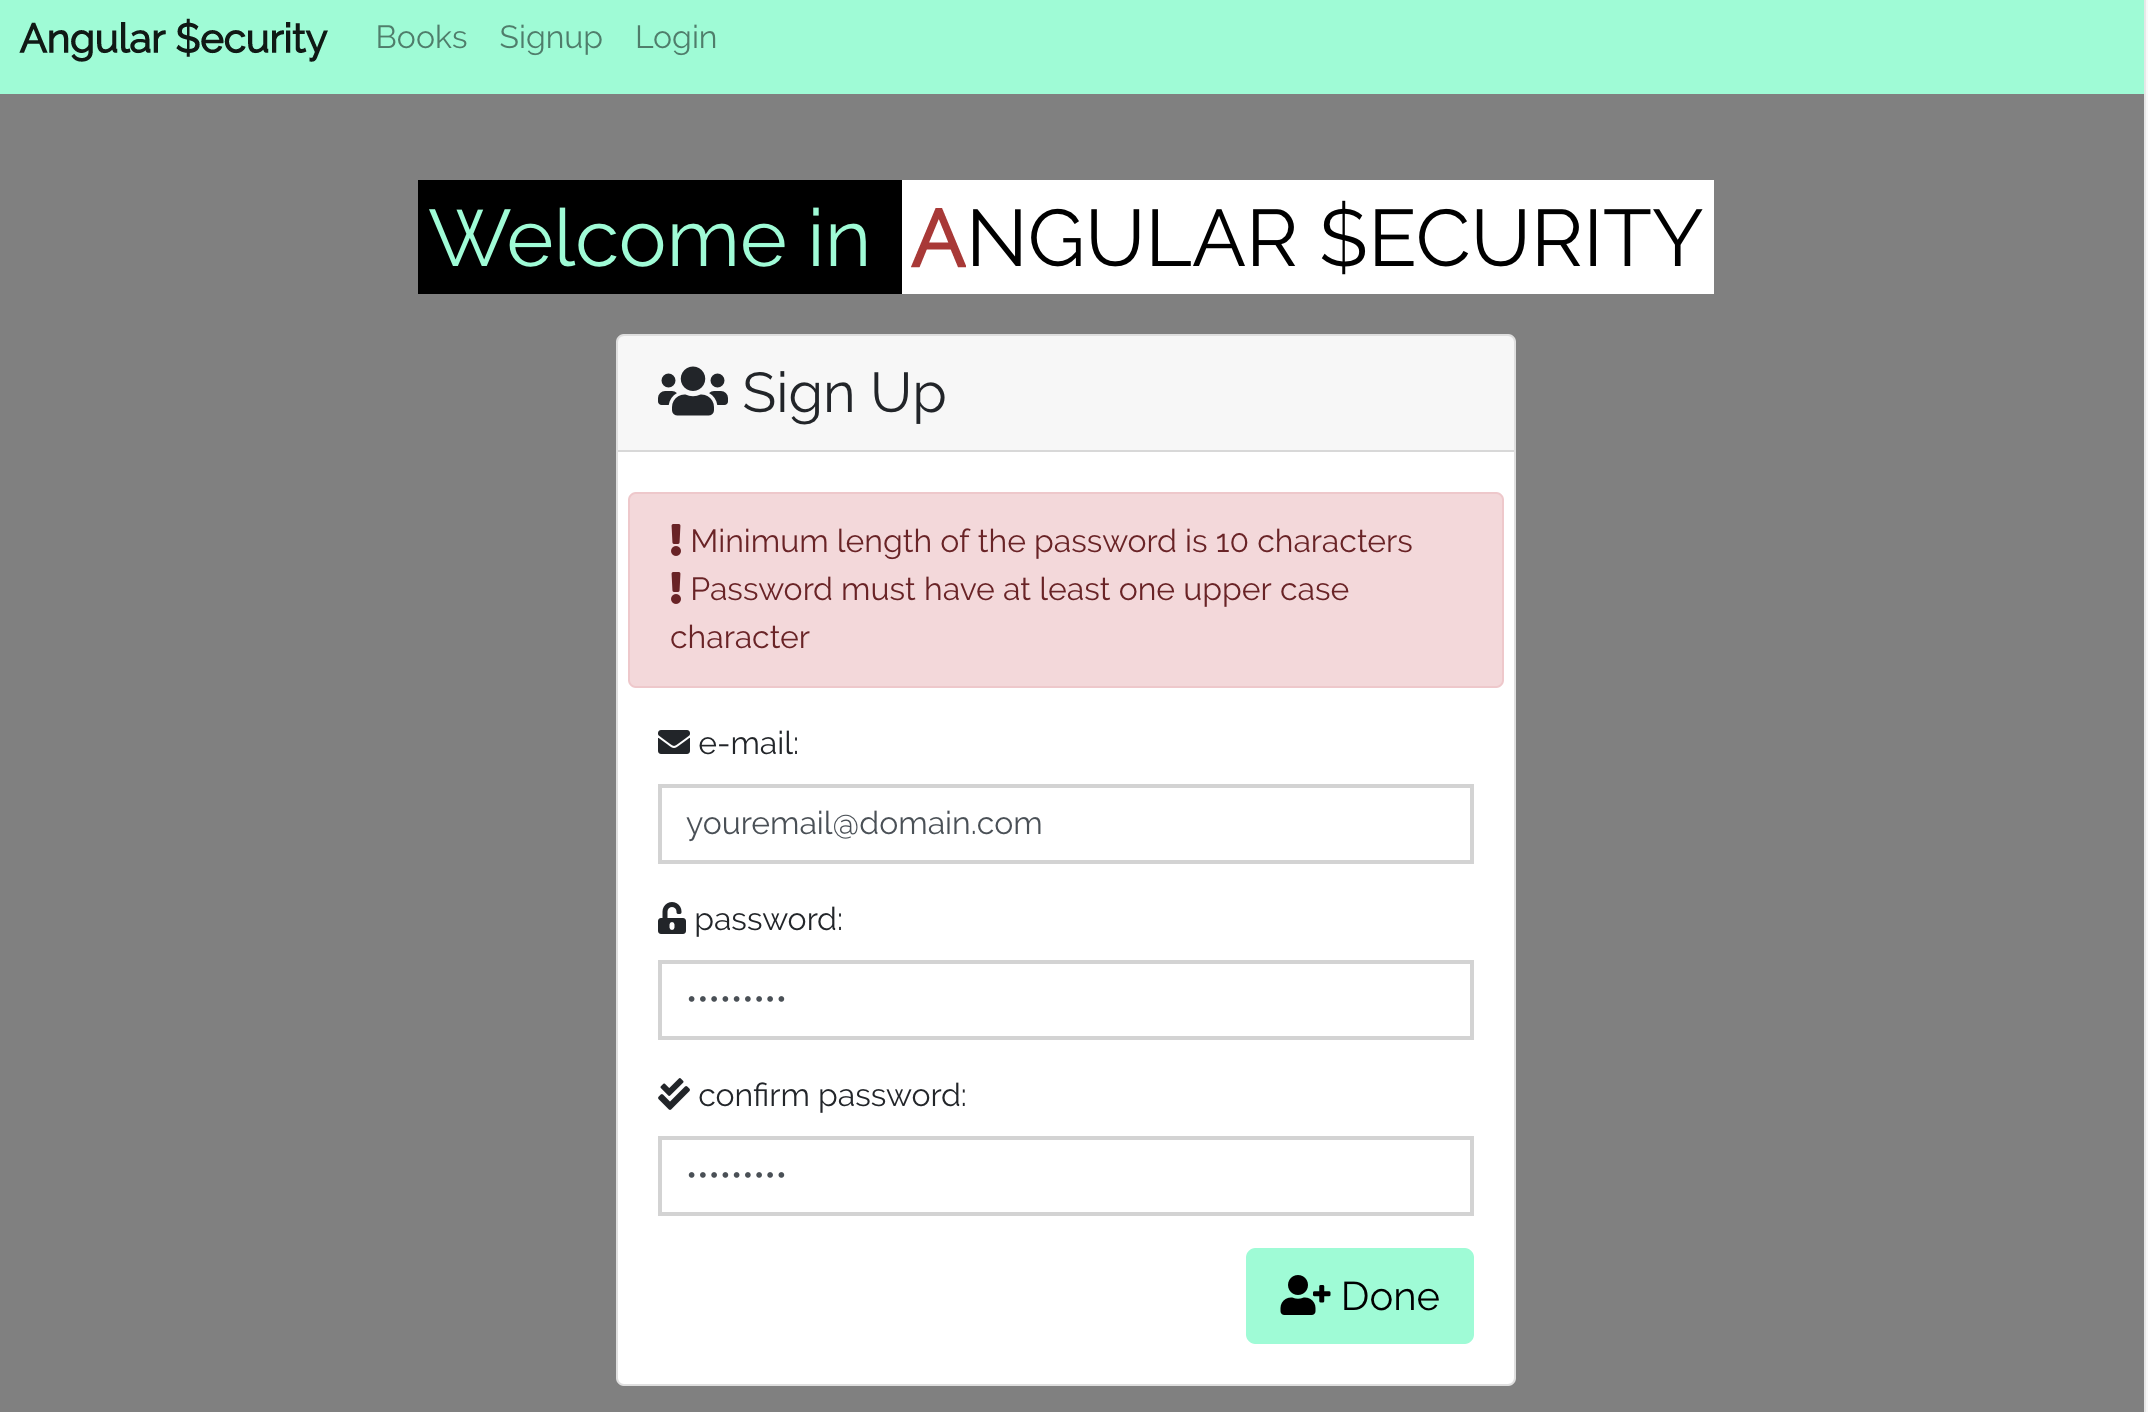
\includegraphics[scale=0.4]{images/security/password-bad-validation.png}
	\caption{Ekran aplikacji pokazowej prezentujący błędną walidację formularza w przypadku podania przez użytkownika haseł, które nie spełniają wymagań zdefiniowanych w schemacie bezpiecznego hasła.}
	\label{Rys:badpassvalid}
\end{figure}

\subsection{Sposób przechowywania haseł użytkowników}
Hasła użytkowników aplikacji przechowywane są w bazie danych w postaci jednokierunkowej funkcji skrótu \textit{Argon2}, która jest zwycięzcą konkursu \textit{Password Hashing Competition} z połowy 2015 roku. Funkcja ta jest rekomendowana przez OWASP (\textit{Open Web Application Security Project}). Jest to globalna, profesjonalna fundacja, która działa charytatywnie. OWASP jest otwarty dla każdego, kto interesuje się bezpieczeństwem nowoczesnych aplikacji internetowych. Organizacja działa na rzecz publikowania artykułów, metodologii, narzędzi i dokumentacji związanych z ochroną danych. 

Funkcja \textit{Argon2} może być używana do mieszania haseł, przechowywania danych uwierzytelniających, pochodnych kluczy lub innych aplikacji. W przeciwieństwie do funkcji \textit{bcrypt} czy \textit{PBKDF2}, \textit{Argon2} cechuje się wysoką adaptacyjnością. Możliwe jest tu bowiem ustawienie aż trzech parametrów: liczby iteracji wykonywanych operacji kryptograficznych, wielkości wykorzystywanej pamięci oraz zrównoleglenia, czyli liczby równoległych wątków działających w tle. Ma ona bardzo prostą konstrukcję umożliwiającą mniejsze zużycie pamięci i efektywne wykorzystanie wielu jednostek obliczeniowych w celu przeprowadzania działań kryptograficznych. Jedną z ciekawych funkcji jest również możliwość sprecyzowania dodawanej soli, długości wyjściowego skrótu czy też możliwość dodania dodatkowego, opcjonalnego klucza. \textit{Argon2} posiada trzy odmiany: \textit{Argon2i}, \textit{Argon2d} oraz \textit{Argon2id}. Funkcja \textit{Argon2d} jest znacznie szybsza od pozostałych i jednocześnie odporna na ataki typu \textit{GPU Cracking}. \textit{Argon2i} charakteryzuje się znacznie większą liczbą odwołań do pamięci co powoduje ją wolniejszą od pozostałych. Zaleca się używanie jej do hashowania haseł. Ostatnia z odmian - \textit{Argon2id} - jest hybrydą dwóch wersji: \textit{Argon2i} oraz \textit{Argon2d}. Czyni ją to odporną na ataki typu \textit{side-channel} i zwiększa jej bezpieczeństwo na metody naruszania zabezpieczeń z użyciem kart graficznych. Ogólna, bardzo uproszczona postać funkcji \textit{Argon2} wygląda następująco:

\begin{verbatim}
ARGON2(password, salt, parallelism, length, memory, count, key)
\end{verbatim}

Jak widać, oprócz przekazania takich parametrów jak hasło czy dodawana sól istnieje równiez możliwość oznaczenia poziomu zrównoleglenia obliczeń (\texttt{parallelism}), określenia ilości pamięci niezbędnej do obliczenia skrótu (\texttt{memory}), określenia opcjonalnego klucza (\texttt{key}) czy też wielkości ciągu wyjściowego (\texttt{count}). Cały algorytm oparty jest o kryptograficzną funkcję skrótu \textit{BLAKE2}, która jest jednym z finalistów konkursu \textit{SHA-3}. 

W autorskiej aplikacji wykorzystano pakiet NPM o nazwie \textit{node-argon2}. Oferuje on większość możliwości, które dostarcza funkcja \textit{argon2}. Funkcja hashowania hasła użytkownika wygląda następująco:

\begin{verbatim}
async function createUserAndSession(res: Response, credentials) {
const passwordDigest = await argon2.hash(credentials.password);
...
}
\end{verbatim}

Jak widać jako parametr funkcji przekazywane jest hasło podane przez użytkownika w trackie rejestracji do serwisu. Rezultat hashowania hasła widoczny jest na zdjęciu \ref{Rys:argon2}.

\begin{figure}[h]
	\centering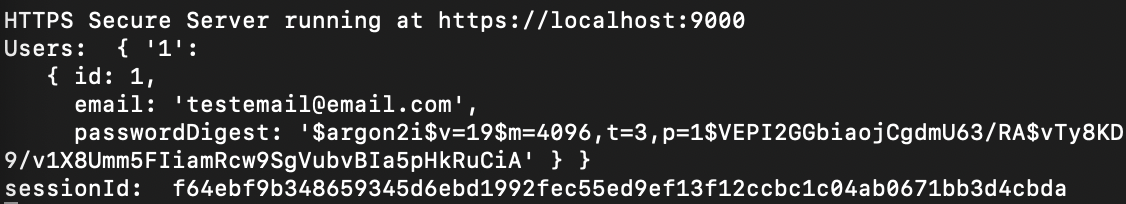
\includegraphics[scale=0.75]{images/security/argon2.png}
	\caption{Okno konsoli serwera po pomyślnej rejestracji nowego użytkownika z wyświetlonym skrótem hasła podanego przez osobę rejestrującą się do serwisu..}
	\label{Rys:argon2}
\end{figure}

Funkcja \texttt{argon2.hash(password, {options})} umożliwia określenie rodzaju funkcji \textit{argon2}. Wystarczy w obiekcie options przekazać wartość \texttt{type: typeOfArgonFunction}. Przykładowy rezultat hashowania hasła \textit{PAssw0rd12} oraz kod źródłowy przedstawione zostały poniżej:

\begin{verbatim}
argon2.hash(password, {type: argon2.argon2id}).then(hash => {
console.log('Argon2id password: ', hash);
}, (err) => {
console.err('An error occured while password hashing: ', err);
});
\end{verbatim}

\begin{figure}[h]
	\centering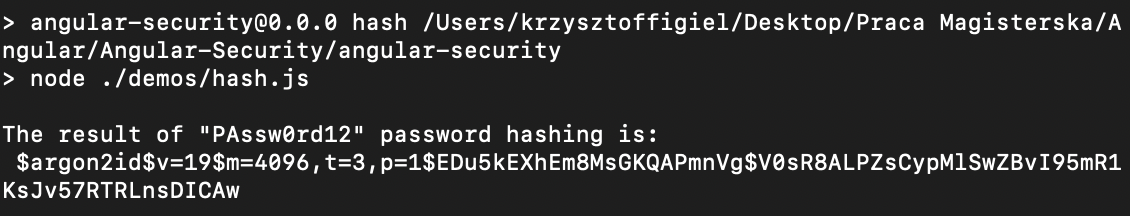
\includegraphics[scale=0.73]{images/security/argon2id.png}
	\caption{Rezultat hashowania hasła \textit{PAssw0rd12} za pomocą funkcji skrótu \textit{Argon2id}.}
	\label{Rys:argon2id}
\end{figure}

Pakiet \textit{node-argon2} oferuje również możliwość weryfikowania hasła. Służy do tego metoda \texttt{argon2.verify('<big long hash>', 'password')}. Rezultat weryfikacji hasła \textit{PAssw0rd12} widoczny jest na zdjęciu \ref{Rys:argon2idmatchfailed}.

\begin{figure}[h]
	\centering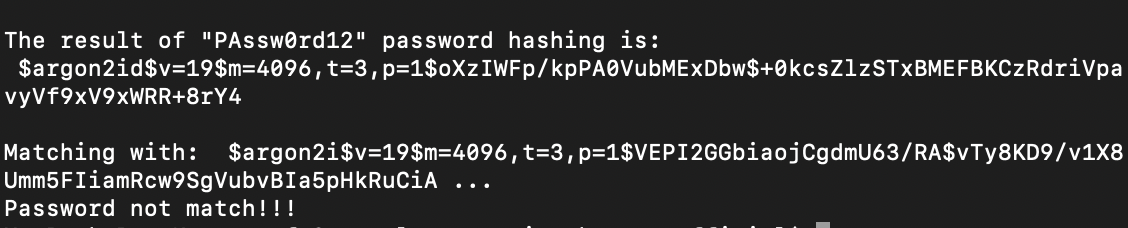
\includegraphics[scale=0.73]{images/security/argon-matching-failed.png}
	\caption{Rezultat wykorzystania funkcji sprawdzającej błędne dopasowanie hasła do funkcji skrótu stworzonego za pomocą \textit{Argon2id}.}
	\label{Rys:argon2idmatchfailed}
\end{figure}

W momencie podstawienia innego skrótu (w tym przypadku skrótu wygenerowanego przez funkcję \textit{argon2i}) metoda program informuje użytkownika o błędnym dopasowaniu hasła. 

\subsection{Mechanizmy podtrzymywania sesji użytkownika}

\subsection{JSON Web Tokens}

\subsection{Metody ochrony aplikacji internetowych przed atakami typu CSRF}

\subsection{Metody ochrony aplikacji internetowych przed atakami typu XSS}


\subsection{Metody ochrony aplikacji internetowych przed atakami typu CSS}

\subsection{Walidacja formularzy}

\subsection{Autoryzacja oparta na rolach użytkowników (RBAC)}

\subsection{Testy aplikacji internetowych z użyciem frameworków Jasmine oraz Karma}


